\chapter{Theoretical Background}
\label{chap:theoretical_background}

This chapter establishes the theoretical, optical, and mathematical foundations underlying passive RGB face presentation attack detection and real-time biometric attendance verification. Building on the problem context introduced in Chapter~\ref{chap:introduction}, it formalizes standardized anti-spoofing taxonomy, analyzes convolutional and normalization mechanics under multi-source domain shifts, reviews candidate detection and recognition algorithms, and motivates the architectural choices developed in Chapter~\ref{chap:methodology}.

\section{Fundamental Concepts}
\label{sec:fundamental_concepts}

\subsection{Presentation Attack Detection Taxonomy}

Within a biometric verification pipeline, Presentation Attack Detection (PAD) evaluates whether a physical target captured by a sensor corresponds to a live human subject (\emph{bona fide presentation}) or an artificial reproduction (\emph{attack presentation}). Under the international standard ISO/IEC 30107-3~\cite{iso30107_3}, Presentation Attack Instruments (PAIs) targeting two-dimensional RGB cameras fall into three primary structural categories, illustrated in Figure~\ref{fig:pad_taxonomy}:
\begin{itemize}
    \item \textbf{Two-dimensional print attacks:} Flat or curved photographs printed via inkjet, laser, or dye-sublimation printers onto matte or glossy paper, occasionally modified by eye-region cutouts.
    \item \textbf{Two-dimensional electronic replay attacks:} Static portraits or pre-recorded video clips displayed on self-illuminated smartphone, tablet, or laptop screens held in front of the verification camera.
    \item \textbf{Composite and three-dimensional artifacts:} Rigid resin masks, flexible silicone masks, or partial screen overlays held adjacent to a live presenter.
\end{itemize}

\begin{figure}[htbp]
\centering
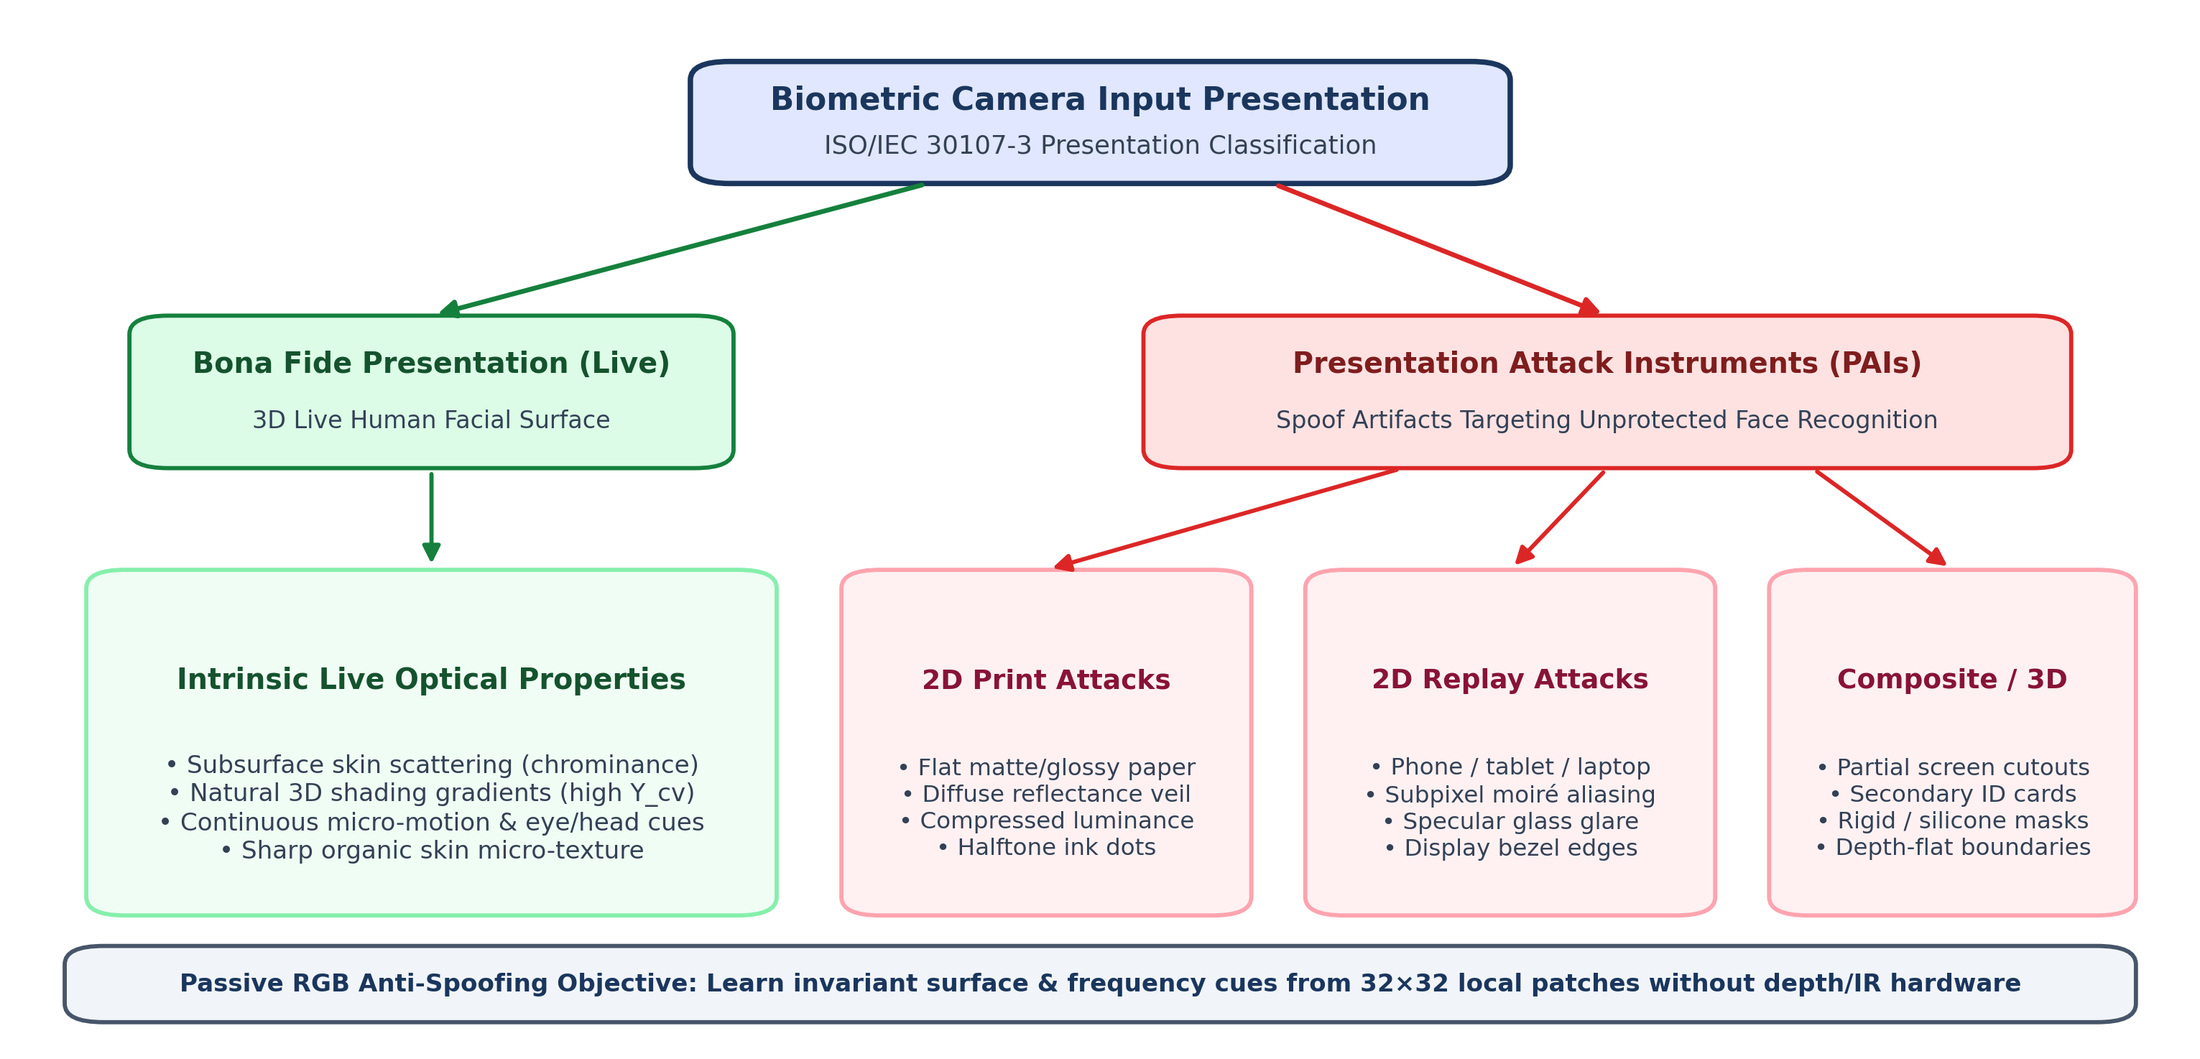
\includegraphics[width=0.96\textwidth]{Images/fig_pad_taxonomy.jpg}
\caption{ISO/IEC 30107-3 biometric presentation classification and passive RGB optical cues distinguishing bona fide faces from presentation attack instruments.}
\label{fig:pad_taxonomy}
\end{figure}

PAD systems are further categorized as \emph{active} or \emph{passive}. Active methods require explicit user participation---such as blinking on cue, turning the head toward a target angle, or reading randomized digits---which increases transaction time and remains vulnerable to edited video replays or deepfake puppetry~\cite{yu2023deep}. Passive PAD operates transparently on incoming video frames, extracting intrinsic physical and frequency-domain signatures within a fraction of a second.

\subsection{Optical and Chrominance Distortion Cues in Monocular RGB}

Although a commodity RGB sensor does not measure metric depth directly, recapturing a face from an intermediate display or paper substrate introduces measurable radiometric distortions~\cite{wen2015face, boulkenafet2016face}:
\begin{enumerate}
    \item \textbf{Subsurface scattering versus planar emission/reflection:} Live human skin is a multi-layered translucent medium in which incident light penetrates the epidermis and scatters through hemoglobin- and melanin-rich dermal layers before exiting. This produces smooth, continuous chrominance transitions in luminance-decoupled spaces such as $YC_rC_b$ and HSV. Conversely, printed paper exhibits a diffuse surface reflectance veil with compressed dynamic range (low luminance coefficient of variation), while electronic screens emit quantized RGB primaries restricted to the display panel's color gamut.
    \item \textbf{Spatial frequency aliasing and moir\'{e} interference:} Projecting discrete display subpixel grids (LCD RGB stripes or OLED PenTile matrices) onto a discrete CMOS camera sensor array generates high-frequency beat patterns (moir\'{e} fringes) and unnatural directional gradients when sampled at close range.
    \item \textbf{Specular glass reflections and planar shading:} Glass-covered mobile displays act as partial mirrors, superimposing sharp specular highlights of indoor ceiling fixtures onto facial regions, whereas three-dimensional facial geometry distributes shading continuously across the nasal bridge, zygomatic arches, and forehead.
\end{enumerate}

\subsection{Single-Stage Face Detection and Open-Set Verification}

A complete biometric attendance system combines three distinct visual tasks: (i) \emph{face detection}, which regresses bounding boxes and facial landmarks across spatial scales to isolate candidate regions of interest (ROIs); (ii) \emph{presentation attack detection}, which estimates the posterior probability that each localized ROI originates from a live face; and (iii) \emph{open-set face verification}, which maps an aligned facial crop onto a unit hypersphere so that identities can be enrolled from reference videos without retraining the recognition backbone~\cite{deng2019arcface}. Separating liveness estimation from identity recognition enables modular upgrades and ensures that spoof rejection remains invariant to whether an attacked identity is newly enrolled.

\section{Mathematical and Theoretical Basis}
\label{sec:mathematical_basis}

\subsection{Convolutional Feature Extraction and Receptive Fields}

Let $\mathbf{X} \in \mathbb{R}^{H \times W \times C_{\text{in}}}$ denote an input tensor of height $H$, width $W$, and channel depth $C_{\text{in}}$ scaled to $[0, 1]$. A two-dimensional discrete convolutional layer parameterized by $C_{\text{out}}$ learnable filter banks $\mathbf{K}^{(m)} \in \mathbb{R}^{k_h \times k_w \times C_{\text{in}}}$ and biases $b^{(m)} \in \mathbb{R}$ computes output feature map $m \in \{1, \dots, C_{\text{out}}\}$ at spatial coordinate $(u, v)$ according to Equation~\eqref{eq:conv2d}:
\begin{equation}
\label{eq:conv2d}
    Z_{u, v, m} = b^{(m)} + \sum_{c=1}^{C_{\text{in}}} \sum_{p=0}^{k_h - 1} \sum_{q=0}^{k_w - 1} X_{s \cdot u + p - P_h,\, s \cdot v + q - P_w,\, c} \, K^{(m)}_{p, q, c},
\end{equation}
where $s$ is the spatial stride and $(P_h, P_w)$ denote zero-padding widths. For kernel size $k$, padding $P$, and stride $s$, the resulting spatial dimension along height (and analogously width) is given by Equation~\eqref{eq:spatial_dim}:
\begin{equation}
\label{eq:spatial_dim}
    H_{\text{out}} = \left\lfloor \frac{H + 2P - k}{s} \right\rfloor + 1.
\end{equation}

Following the architectural principle established by Simonyan and Zisserman~\cite{simonyan2015very}, stacking two consecutive $3\times3$ convolutional layers with unit stride ($s=1$) yields an effective $5\times5$ receptive field while inserting an intermediate nonlinear activation and requiring only $2 \times (3^2 C^2) = 18 C^2$ weights instead of $5^2 C^2 = 25 C^2$. Pointwise nonlinearity is introduced via the Rectified Linear Unit (ReLU) in Equation~\eqref{eq:relu}:
\begin{equation}
\label{eq:relu}
    \phi(z) = \max(0, z),
\end{equation}
which preserves non-vanishing unit gradients in the positive half-space while inducing sparse activations. Overfitting on compact datasets is mitigated during training via inverted Dropout~\cite{srivastava2014dropout}, which multiplies hidden activations by independent Bernoulli masks $r_j \sim \text{Bernoulli}(1 - p_{\text{drop}})$ scaled by $(1 - p_{\text{drop}})^{-1}$.

At the classification head, raw logits $\mathbf{g} = [g_{\text{fake}}, g_{\text{real}}]^\top \in \mathbb{R}^2$ are mapped onto the probability simplex via the Softmax operator in Equation~\eqref{eq:softmax}:
\begin{equation}
\label{eq:softmax}
    P(y = c \mid \mathbf{X}) = \hat{y}_c = \frac{\exp(g_c)}{\sum_{k \in \{\text{fake}, \text{real}\}} \exp(g_k)}, \quad c \in \{\text{fake}, \text{real}\}.
\end{equation}
Given one-hot ground-truth targets $\mathbf{y}_i = [y_{i,0}, y_{i,1}]^\top \in \{0, 1\}^2$ across a mini-batch of $B$ crops and optional non-negative sample weights $w_i > 0$, parameters $\theta$ are optimized by minimizing the weighted categorical cross-entropy loss in Equation~\eqref{eq:cce}:
\begin{equation}
\label{eq:cce}
    \mathcal{L}_{\text{CCE}}(\theta) = -\frac{1}{B} \sum_{i=1}^{B} w_i \sum_{c=0}^{1} y_{i,c} \log \left(\hat{y}_{i,c}(\mathbf{X}_i; \theta)\right).
\end{equation}

\subsection{Feature Normalization Under Multi-Source Covariate Shift}

Internal activation distributions shift continuously during gradient-based training. Batch Normalization (BN)~\cite{ioffe2015batch} standardizes each channel $c$ across the mini-batch and spatial grid $\Omega = \{1, \dots, H\} \times \{1, \dots, W\}$ of cardinality $M = B \cdot H \cdot W$:
\begin{equation}
\label{eq:batchnorm}
    \mu_{\mathcal{B}, c} = \frac{1}{M} \sum_{i=1}^{B} \sum_{(u,v) \in \Omega} Z^{(i)}_{u,v,c}, \qquad
    \sigma^2_{\mathcal{B}, c} = \frac{1}{M} \sum_{i=1}^{B} \sum_{(u,v) \in \Omega} \left(Z^{(i)}_{u,v,c} - \mu_{\mathcal{B}, c}\right)^2,
\end{equation}
followed by an affine transformation $\tilde{Z}^{(i)}_{u,v,c} = \gamma_c (Z^{(i)}_{u,v,c} - \mu_{\mathcal{B}, c}) / \sqrt{\sigma^2_{\mathcal{B}, c} + \epsilon} + \beta_c$ with learnable scale $\gamma_c$ and shift $\beta_c$. Crucially, during training BN maintains exponential moving averages (EMA) for test-time inference according to Equation~\eqref{eq:bn_ema}:
\begin{equation}
\label{eq:bn_ema}
    \bar{\mu}_c^{(t)} = \alpha \, \bar{\mu}_c^{(t-1)} + (1 - \alpha)\, \mu_{\mathcal{B}, c}^{(t)}, \qquad
    \bar{\sigma}_c^{2\,(t)} = \alpha \, \bar{\sigma}_c^{2\,(t-1)} + (1 - \alpha)\, \sigma_{\mathcal{B}, c}^{2\,(t)},
\end{equation}
where $\alpha \in (0, 1)$ is the momentum coefficient (typically $0.99$).

Equations~\eqref{eq:cce}--\eqref{eq:bn_ema} expose a critical failure mechanism when merging imbalanced multi-camera datasets: scalar loss weights $w_i$ rescale parameter gradients $\nabla_\theta \mathcal{L}_{\text{CCE}}$ toward minority-domain samples, yet $\mu_{\mathcal{B}, c}$ and $\sigma^2_{\mathcal{B}, c}$ in Equation~\eqref{eq:batchnorm} remain \emph{unweighted} arithmetic averages dominated by the majority source. Consequently, convolutional weights co-adapt to batch-normalized activations whose statistics reflect the majority camera, producing severe threshold miscalibration at inference time.

Group Normalization (GN)~\cite{wu2018group} eliminates batch-composition dependence entirely by partitioning the $C$ channels of each individual sample $i$ into $G$ groups and normalizing strictly within sample-local index sets $\mathcal{S}_{i, g} = \{(u, v, k) : (u, v) \in \Omega,\, \lfloor k / (C/G) \rfloor = g\}$:
\begin{equation}
\label{eq:groupnorm}
    \mu_{\text{GN}}(i, g) = \frac{1}{|\mathcal{S}_{i,g}|} \sum_{(u,v,k) \in \mathcal{S}_{i,g}} Z^{(i)}_{u,v,k}, \qquad
    \sigma^2_{\text{GN}}(i, g) = \frac{1}{|\mathcal{S}_{i,g}|} \sum_{(u,v,k) \in \mathcal{S}_{i,g}} \left(Z^{(i)}_{u,v,k} - \mu_{\text{GN}}(i, g)\right)^2.
\end{equation}
For one-dimensional dense layers where spatial dimensions collapse ($H=W=1$), setting $G=1$ recovers Layer Normalization (LN)~\cite{ba2016layer}, computing statistics identically during training and single-sample inference without moving averages.

\subsection{Adaptive Optimization and Weight-Space Interpolation}

Network parameters are updated via the Adam optimizer~\cite{kingma2015adam}, which tracks bias-corrected first and second gradient moments $(\hat{\mathbf{m}}_t, \hat{\mathbf{v}}_t)$ with decay rates $(\beta_1, \beta_2)$ and step size $\eta$ as shown in Equation~\eqref{eq:adam}:
\begin{equation}
\label{eq:adam}
    \mathbf{m}_t = \beta_1 \mathbf{m}_{t-1} + (1 - \beta_1)\mathbf{g}_t, \quad
    \mathbf{v}_t = \beta_2 \mathbf{v}_{t-1} + (1 - \beta_2)\mathbf{g}_t^{\odot 2}, \quad
    \theta_t = \theta_{t-1} - \eta \frac{\mathbf{m}_t / (1 - \beta_1^t)}{\sqrt{\mathbf{v}_t / (1 - \beta_2^t)} + \epsilon}.
\end{equation}

When adapting a broadly trained anchor model $\theta_{\text{anchor}}$ to a specialized target-camera distribution yielding fine-tuned weights $\theta_{\text{ft}}$, unconstrained fine-tuning can erode out-of-distribution robustness on secondary cameras. Weight-Space Ensembling for Fine-Tuning (WiSE-FT)~\cite{wortsman2022robust} linearly interpolates parameters within shared basin geometry according to Equation~\eqref{eq:wiseft}:
\begin{equation}
\label{eq:wiseft}
    \theta^*(\lambda) = (1 - \lambda)\,\theta_{\text{anchor}} + \lambda\,\theta_{\text{ft}}, \quad \lambda \in [0, 1],
\end{equation}
achieving target-domain accuracy gains while retaining multi-camera invariance at zero additional inference cost.

\subsection{Optical Quality, Spatial Tracking, Verification, and PAD Metrics}

\noindent\textbf{Defocus Estimation:} Motion and out-of-focus blur attenuate high-frequency screen moir\'{e} and skin pore cues, causing blurred bona fide faces to resemble low-resolution replays. Sharpness on a grayscale crop $I_g$ is quantified by the variance of the discrete Laplacian operator~\cite{pech2000diatom} in Equation~\eqref{eq:laplacian}:
\begin{equation}
\label{eq:laplacian}
\begin{aligned}
    \nabla^2 I_g(u, v) &= I_g(u+1,v) + I_g(u-1,v) + I_g(u,v+1) + I_g(u,v-1) - 4I_g(u,v), \\
    \sigma^2_{\text{Lap}} &= \text{Var}_{u,v}\!\left(\nabla^2 I_g(u,v)\right).
\end{aligned}
\end{equation}

\noindent\textbf{Bounding-Box Association:} Across consecutive video frames, detected face boxes $B_a = (x_1^a, y_1^a, x_2^a, y_2^a)$ and active tracks $B_b = (x_1^b, y_1^b, x_2^b, y_2^b)$ are matched via Intersection-over-Union ($\text{IoU}$) in Equation~\eqref{eq:iou}:
\begin{equation}
\label{eq:iou}
    \text{IoU}(B_a, B_b) = \frac{\max(0, \min(x_2^a, x_2^b) - \max(x_1^a, x_1^b)) \cdot \max(0, \min(y_2^a, y_2^b) - \max(y_1^a, y_1^b))}{\text{Area}(B_a) + \text{Area}(B_b) - \text{Area}(B_a \cap B_b)}.
\end{equation}

\noindent\textbf{Angular-Margin Verification:} For identity recognition, ArcFace~\cite{deng2019arcface} normalizes both embedding vectors $\hat{\mathbf{e}}_i = \mathbf{e}_i / \|\mathbf{e}_i\|_2 \in \mathbb{R}^{512}$ and class weight centers $\hat{\mathbf{W}}_j = \mathbf{W}_j / \|\mathbf{W}_j\|_2$, enforcing an additive angular margin penalty $m$ with feature scale $s$ during backbone pretraining (Equation~\eqref{eq:arcface}):
\begin{equation}
\label{eq:arcface}
    \mathcal{L}_{\text{Arc}} = -\frac{1}{N} \sum_{i=1}^{N} \log \frac{\exp\!\left(s \cos(\theta_{y_i} + m)\right)}{\exp\!\left(s \cos(\theta_{y_i} + m)\right) + \sum_{j \neq y_i} \exp\!\left(s \cos \theta_j\right)}, \quad \theta_j = \arccos\!\left(\hat{\mathbf{W}}_j^\top \hat{\mathbf{e}}_i\right).
\end{equation}
At attendance inference time, matching a query embedding $\hat{\mathbf{q}}$ against a gallery of $\ell_2$-normalized prototype vectors $\{\hat{\mathbf{p}}_k\}_{k=1}^{K}$ reduces to maximum inner-product cosine similarity in Equation~\eqref{eq:cosine_sim}:
\begin{equation}
\label{eq:cosine_sim}
    s_{\max}(\hat{\mathbf{q}}) = \max_{1 \le k \le K} \left(\hat{\mathbf{q}}^\top \hat{\mathbf{p}}_k\right),
\end{equation}
accepting the identity associated with the winning prototype if and only if $s_{\max}(\hat{\mathbf{q}}) \ge \tau$ and the upstream anti-spoofing gate classifies the presentation as bona fide.

\noindent\textbf{ISO/IEC 30107-3 PAD Error Rates:} Letting $\text{TP}_{\text{real}}$ and $\text{FN}_{\text{real}}$ denote bona fide presentations classified as real and fake, and letting $\text{TN}_{\text{fake}}$ and $\text{FP}_{\text{fake}}$ denote spoof attacks classified as fake and real, standardized PAD performance is governed by Attack Presentation Classification Error Rate ($\text{APCER}$), Bona Fide Presentation Classification Error Rate ($\text{BPCER}$), and Average Classification Error Rate ($\text{ACER}$) in Equation~\eqref{eq:iso_metrics}:
\begin{equation}
\label{eq:iso_metrics}
    \text{APCER} = \frac{\text{FP}_{\text{fake}}}{\text{TN}_{\text{fake}} + \text{FP}_{\text{fake}}}, \quad
    \text{BPCER} = \frac{\text{FN}_{\text{real}}}{\text{TP}_{\text{real}} + \text{FN}_{\text{real}}}, \quad
    \text{ACER} = \frac{\text{APCER} + \text{BPCER}}{2}.
\end{equation}

\section{Existing Frameworks and Algorithms}
\label{sec:exist_frameworks_algorithms}

Deploying an integrated real-time anti-spoofing and attendance pipeline requires selecting compatible face detectors, PAD classifiers, recognition backbones, and CPU execution runtimes. Table~\ref{tab:algorithms} compares the principal algorithmic candidates across these four layers.

\begin{table}[htbp]
\centering
\caption{Technical comparison of candidate detection, anti-spoofing, verification, and inference frameworks.}
\label{tab:algorithms}
\footnotesize
\begin{tabular}{L{2.8cm}L{2.3cm}L{4.3cm}L{4.5cm}}
\toprule
\textbf{Algorithm / Engine} & \textbf{Subsystem} & \textbf{Technical Advantages} & \textbf{Constraints / Trade-offs} \\
\midrule
ResNet-10 SSD~\cite{liu2016ssd} & Face Detection & Consistent tight facial crop geometry on $300\times300$ inputs; mature OpenCV Caffe DNN support. & Lacks native 5-point landmarks; higher false positives on background clutter than anchor-free detectors. \\
\addlinespace[1.5pt]
YuNet ONNX~\cite{wu2023yunet} & Face Detection & Tiny footprint ($<250$~KB); millisecond CPU latency; outputs 5 facial landmarks for eye-span quality checks. & Slightly looser default bounding-box margins than Caffe SSD unless aligned. \\
\addlinespace[1.5pt]
SCRFD~\cite{guo2022scrfd} & Face Detection & Computation redistribution yields high recall across scales; paired natively with InsightFace alignment. & Bounding-box aspect ratio differs from SSD/YuNet crops, requiring ROI re-alignment before PAD scoring. \\
\addlinespace[1.5pt]
Colour-LBP~\cite{boulkenafet2016face} & Face PAD & Handcrafted $YC_bC_r$/HSV histograms; zero GPU requirement; transparent feature space. & Degrades sharply on high-density OLED panels and uncalibrated webcam AWB shifts. \\
\addlinespace[1.5pt]
CDCN~\cite{yu2020searching} / Aux-Depth~\cite{liu2018learning} & Face PAD & Captures fine-grained central gradient differences and pseudo-3D facial curvature. & Dense $32\times32$ depth supervision and multi-level fusion incur substantial CPU latency per frame. \\
\addlinespace[1.5pt]
PatchNet~\cite{wang2022patchnet} & Face PAD & Enforces local surface patch discrimination; resists global subject identity memorization. & Requires center-crop/scale-jitter pretext formulation and ResNet-18-scale backbone compute. \\
\addlinespace[1.5pt]
\texttt{LivenessNet} (VGG-style~\cite{simonyan2015very}) & Face PAD & $545{,}154$ parameters ($2.15$~MiB); $32\times32$ patch input inherently suppresses identity detail; $0.163$~ms CPU inference. & Small receptive scale lacks global context (e.g., hand holding phone bezel) unless paired with temporal/ROI logic. \\
\addlinespace[1.5pt]
ArcFace (ResNet-50)~\cite{deng2019arcface} & Verification & Geodesic angular margin yields highly separable $512$-D unit embeddings for few-shot video enrollment. & Completely vulnerable to 2D print and screen replay without an external PAD gate. \\
\addlinespace[1.5pt]
LiteRT + XNNPACK~\cite{david2021tensorflow} & CPU Runtime & Fuses Conv+BN layers into static flatbuffers; vectorizes $3\times3$ kernels on x86 AVX2/FMA CPUs. & Requires static graph freezing; dynamic Python training callbacks are unavailable post-export. \\
\bottomrule
\end{tabular}
\end{table}

\subsection{Face Detection Frameworks}

Single Shot MultiBox Detector (SSD)~\cite{liu2016ssd} with a reduced ResNet-10 backbone processes $300\times300$ mean-subtracted BGR blobs and produces stable, tightly cropped facial boxes well suited for offline training crop generation. For live streaming and quality gating, YuNet~\cite{wu2023yunet} employs depthwise separable convolutions and an anchor-free head to regress both bounding boxes and five facial keypoints (left/right eye centers, nose tip, mouth corners) in a few milliseconds on CPU. Within the attendance recognition stack, Sample and Computation Redistribution for Face Detection (SCRFD)~\cite{guo2022scrfd} reallocates FLOPs toward shallow feature pyramid stages, supplying accurate 5-point landmarks for similarity-transform alignment into $112\times112$ ArcFace inputs.

\subsection{Passive Anti-Spoofing Architectures and Runtime Compilers}

While deep auxiliary networks such as CDCN~\cite{yu2020searching} and multi-channel CNNs~\cite{george2020biometric} excel on GPU benchmarks, CPU-bound attendance kiosks benefit from compact VGG-style~\cite{simonyan2015very} or MobileNetV3-style~\cite{howard2019searching} designs operating on low-resolution facial patches. Consistent with the patch-level hypothesis of PatchNet~\cite{wang2022patchnet}, downsampling a localized face box to $32\times32$~pixels discards fine biometric identity structures (such as iris patterns or mole placement) while retaining macro-radiometric and screen-aliasing cues across color channels. Furthermore, compiling a Keras convolutional graph into a frozen LiteRT (\texttt{.tflite}) model~\cite{david2021tensorflow} folds Batch Normalization scale and offset parameters directly into preceding convolution weights, eliminating Python dispatch overhead and enabling sub-millisecond SIMD execution via XNNPACK.

\section{Limitations and Research Motivation}
\label{sec:limitations_motivation}

Synthesizing the theoretical analysis in Section~\ref{sec:mathematical_basis} and the framework survey in Section~\ref{sec:exist_frameworks_algorithms} reveals four concrete failure modes that frequently undermine lightweight passive anti-spoofing systems in practice:
\begin{enumerate}
    \item \textbf{Optimistic evaluation via frame-level leakage:} Adjacent frames extracted from a $30$~FPS video share nearly identical background illumination, subject identity, and sensor noise. Random frame-level train/test splits allow compact CNNs to memorize session-specific color casts, reporting $>99\%$ laboratory accuracy while failing on unseen subjects ($\text{ACER} > 25\%$).
    \item \textbf{Normalization drift in multi-source training:} Combining a large legacy webcam archive with smaller target-camera recordings using inverse-frequency sample weights introduces severe mismatch between unweighted Batch Normalization moving statistics (Equation~\eqref{eq:bn_ema}) and weighted gradient updates (Equation~\eqref{eq:cce}).
    \item \textbf{Detector geometry and compression confounding:} Mixing videos across file containers (\texttt{.mov} vs.\ \texttt{.mp4}) or swapping face detectors between training (SSD) and deployment (SCRFD) introduces spurious domain shortcuts and crop-scale shifts that degrade live recognition gating.
    \item \textbf{Single-frame decision volatility:} Evaluating Equation~\eqref{eq:softmax} independently on every video frame exposes interactive check-in terminals to momentary specular glare and motion blur, causing rapid label oscillation or transient false accepts.
\end{enumerate}

Addressing the first three challenges requires a disciplined data acquisition, optical filtering, and person-disjoint partitioning pipeline before any model optimization takes place. Chapter~\ref{chap:data_processing} details how raw video streams were collected, cleaned, audited, and structured to establish a leakage-free foundation.
